% !TEX root = ../../main.tex

\chapter{The Mutex Watershed Algorithm}
Image partitioning, or segmentation without semantics, is the task of decomposing an image into distinct segments, or equivalently to detect closed contours. Most prior work either requires seeds, one per segment; or a threshold; or formulates the task as multicut / correlation clustering, an NP-hard problem. Here, we propose an \REVIEW{efficient} algorithm for \REVIEW{graph partitioning}, the ``Mutex Watershed''. Unlike seeded watershed, the algorithm can accommodate not only attractive but also repulsive cues, allowing it to find a previously \emph{unspecified} number of segments without the need for explicit seeds or a tunable threshold. We also prove that this simple algorithm solves to global optimality an objective function that is intimately related to the multicut / correlation clustering integer linear programming formulation. 
The algorithm is deterministic, very simple to implement, and has empirically linearithmic complexity. 
%It can be related to with empirically linearithmic complexity. %Just like multicut / correlation clustering or modularity clustering, it determines an optimal number of segments automatically; but unlike these criteria, ours exhibits matroid structure and can be optimized globally by a simple greedy algorithm akin to a minimal spanning tree computation. 
%The algorithm itself, which we dub ``Mutex Watershed'', is closely related to a minimal spanning tree computation. It is deterministic and easy to implement. 
When presented with short-range attractive and long-range repulsive cues from a deep neural network, the Mutex Watershed gives the best results currently known for the %define the state-of-the-art in the 
competitive ISBI 2012 EM segmentation benchmark.

\section{Introduction}\label{intro}
Most image partitioning algorithms are defined over a graph encoding purely attractive interactions. No matter whether a segmentation or clustering is then found agglomeratively (as in single linkage clustering / watershed) or divisively (as in spectral clustering or iterated normalized cuts), the user either needs to specify the desired number of segments or a termination criterion. An even stronger form of supervision is in terms of seeds, where one pixel of each segment needs to be designated either by a user or automatically. Unfortunately, clustering with 
% First paragraph: watershed intro
%The watershed algorithm is a key tool for many image segmentation tasks. It is especially suitable for objects with
%high surface-to-volume ratio, because it does not induce a shrinking bias, in contrast to multi-terminal cuts or (conditional) random fields. The classical watershed pipeline consists of three steps: computation of a boundary map, seed definition, and region assignment. 
% Second paragraph: learning in watershed
%Machine learning has dramatically improved the quality of the resulting segmentations. Most authors \cite{???} apply learning to the first step: they construct target boundary maps from ground truth segmentations and train neural networks to reproduce these maps as precisely as possible. %Recently, \cite{???} demonstrated that segmentation quality can be further improved by joint end-to-end training of boundary map estimation and region assignment. This approach affords {\em dynamic} boundary map calculations, which take the current partial segmentation state into account in order to improve subsequent assigment decisions. 
% Third paragraph: the difficulty of seeding
automated seed selection remains a fragile and error-fraught process, because every missed or hallucinated seed causes an under- or oversegmentation error. Although the learning of good edge detectors boosts the quality of classical seed selection strategies (such as finding local minima of the boundary map, or thresholding boundary maps), non-local effects of seed placement along with strong variability in region sizes and shapes make it hard for any learned predictor to place {\em exactly one} seed in every true region.

In contrast to the above class of algorithms, multicut / correlation clustering partitions vertices with both attractive and repulsive interactions encoded into the edges of a graph. Multicut has the great advantage that a ``natural'' partitioning of a graph can be found, without needing to specify a  desired number of clusters, or a termination criterion, or one seed per region. Its great drawback is that its optimization is NP-hard. 
% Fourth paragraph: introduce auxiliary repulsive edges

The main insight of this paper is that when both attractive and repulsive interactions between pixels are available, then a generalization of the watershed algorithm can be devised that segments an image {\em without} the need for seeds or stopping criteria or thresholds. It examines all graph edges, attractive and repulsive, sorted by their weight and adds these to an active set iff they are not in conflict with previous, higher-priority, decisions. The attractive subset of the resulting active set  is a forest, with one tree representing each segment. However, the active set can have loops involving more than one repulsive edge.
 See Fig.~\ref{fig:main} for a visual abstract. 
%Figure two (TODO reference to fig 1). %Importantly, the strengths of the repulsive edges can be learned in the same way as, and jointly with, the affinities of the original edges by minimizing a structured loss similar to \cite{???}.

In summary, our principal contributions are, first, 
a fast deterministic algorithm for \REVIEW{graph partitioning with both positive and negative edge weights} that does not need prior specification of the number of clusters~(section \ref{sec:MWS_objective}); and second, its theoretical characterization, including proof that it globally optimizes an objective related to the multicut correlation clustering objective~(\ref{sec:MWS_objective}).

Combined with a deep net, the algorithm also happens to define the state-of-the-art in a competitive neuron segmentation challenge~(\autoref{4_results}).

This is an extended version version of \cite{wolf2018mutex}, with the second principal contribution (section \ref{sec:MWS_objective}) being new.


\begin{figure}[t]
    \centering
    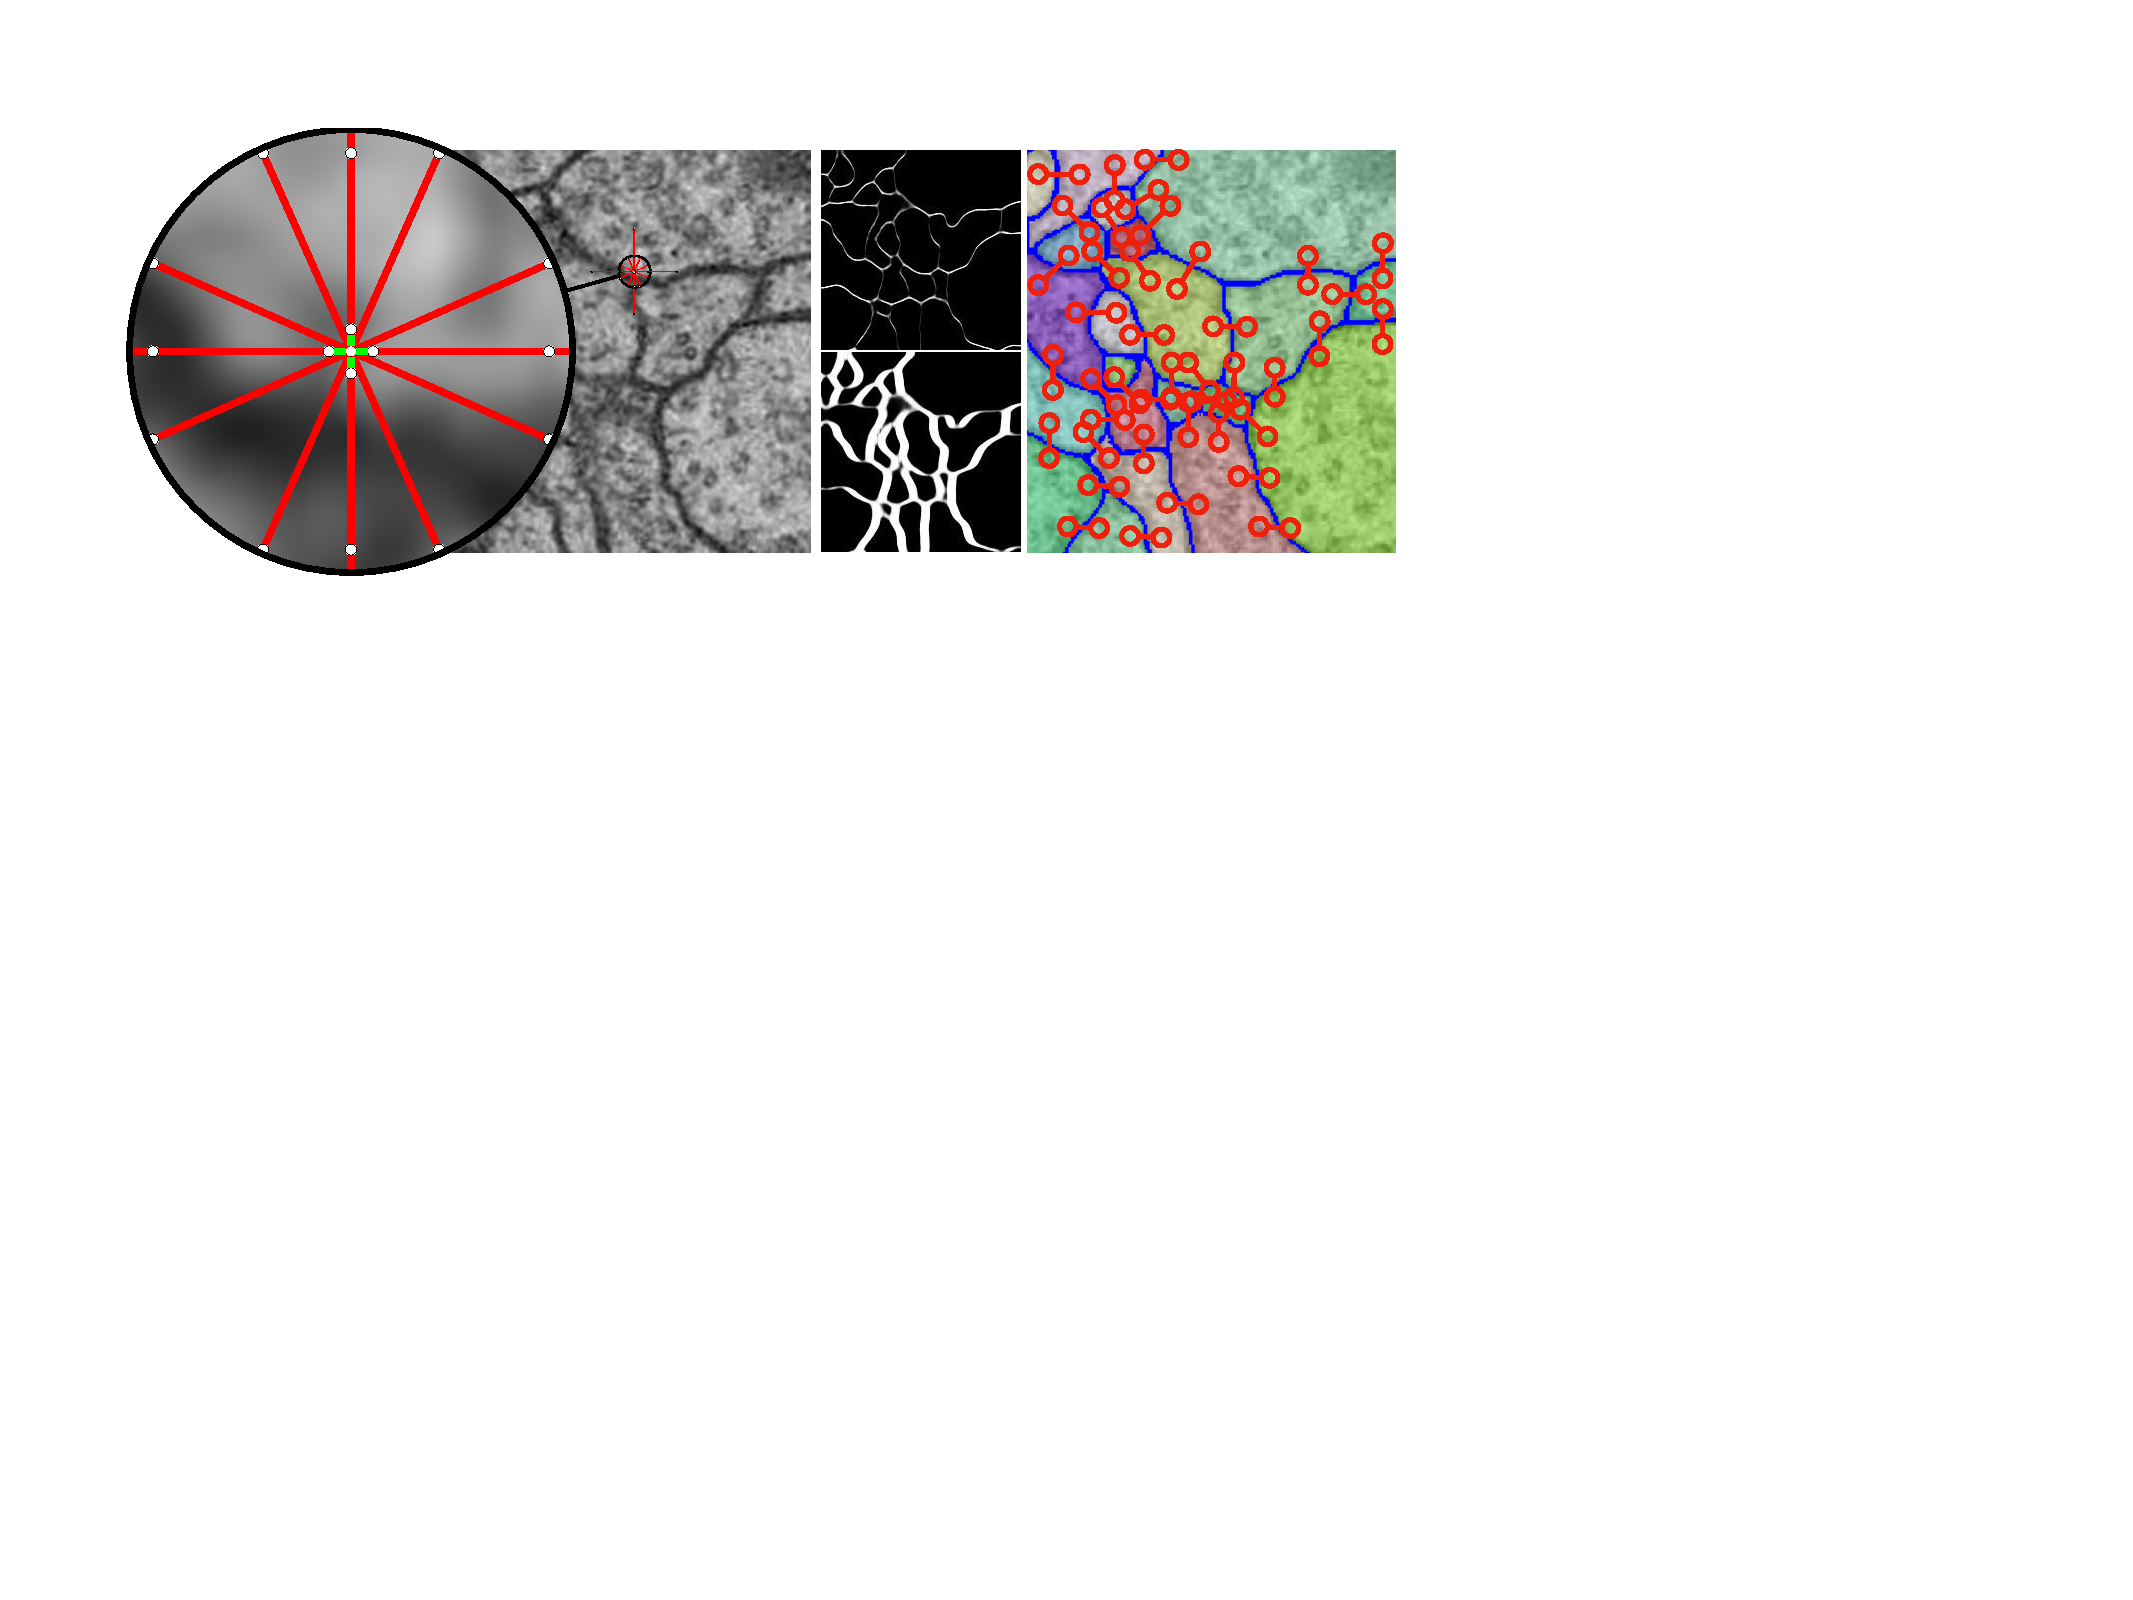
\includegraphics[width=1.\linewidth]{figures/MWS/images/fig1slimt.pdf}%
    % \begin{tabular}{cc}
    % \includegraphics[width=0.1\linewidth, valign=t]{images/affp0p0p-1pzp6.jpg}%
    % \includegraphics[width=0.1\linewidth, valign=t]{images/affp0p-9p0pzp6.jpg}\\
    % \includegraphics[width=0.1\linewidth, valign=t]{images/affp-1p1p-1pzp6.jpg}%
    % \includegraphics[width=0.1\linewidth, valign=t]{images/affp0p0p-9.jpg}\\   
    % \end{tabular}
    % \includegraphics[width=0.2\linewidth, valign=t]{images/affp0p0p-9.jpg}
    % \includegraphics[width=0.3\linewidth]{images/U-Net.pdf}%
    % \includegraphics[width=0.3\linewidth, valign=t]{images/fig_1_seg.png}
    \caption{Left: Overlay of raw data from the ISBI 2012 EM segmentation challenge and the edges for which attractive (green) or repulsive (red) interactions are estimated for each pixel using a CNN. Middle: vertical / horizontal repulsive interactions at intermediate / long range are shown in the top / bottom half. Right: Active mutual exclusion (mutex) constraints that the proposed algorithm invokes during the segmentation process.}
    \label{fig:main}
    \vspace{-0.05cm}
\end{figure}

